\setcounter{section}{4}
\section{Bild und Kern}

\subsection{Bild}

Ganz am Anfang der Linearen Algebra I sahen wir, wie die Matrix-Vektor-Multiplikation ausgeführt wird. Wir können diese Multiplikation, einer Matrix \( A \) mit einem Vektor \( x \), auch als Linearkombination der Spaltenvektoren von \( A \) ausdrücken

\begin{equation*}
    \begin{pmatrix}
        a_{11} & a_{12} & a_{13} \\
        a_{21} & a_{22} & a_{23} \\
        a_{31} & a_{32} & a_{33} \\
    \end{pmatrix}
    \begin{pmatrix}
        x_1 \\
        x_2 \\
        x_3 \\
    \end{pmatrix} =   
    \begin{pmatrix}
        a_{11} \\
        a_{21} \\
        a_{31} \\
    \end{pmatrix} x_1 +
    \begin{pmatrix}
        a_{12} \\
        a_{22} \\
        a_{32} \\
    \end{pmatrix} x_2 +
    \begin{pmatrix}
        a_{13} \\
        a_{23} \\
        a_{33} \\
    \end{pmatrix} x_3.
\end{equation*}

\vspace{0.5\baselineskip}

Das heisst, dass alle möglichen Ergebnisse einer Matrix-Vektor-Multiplikation \( Ax \) durch die Linearkombination der Spaltenvektoren von \( A \) dargestellt werden können. Die Menge aller dieser Ergebnisse nennt sich Bild. Mathematisch ist das Bild einer Matrix \( A \in \mathbb{R}^{m \times n} \) durch

\begin{equation*}
    \text{Bild}(A) = \{ y \in \mathbb{R}^m  \mid  \exists \ x \in \mathbb{R}^n \ \text{sodass} \ y = Ax \}
\end{equation*}

\vspace{0.25\baselineskip}

definiert. Grafisch können wir uns das Bild gut im zweidimensionalen Raum vorstellen. Seien beispielsweise die Matrizen

\begin{equation*}
    A = \begin{pmatrix}
        1 & 2 \\
        2 & 0 \\
    \end{pmatrix} \qquad \text{und} \qquad B = \begin{pmatrix}
        1 & 2 \\
        2 & 4 \\
    \end{pmatrix}
\end{equation*}

\vspace{0.25\baselineskip}

gegeben. Wir können nun grafisch die Bilder von \( A \) und \( B \) darstellen. 

\begin{figure}[h]
    \centering
    \tikzset{every picture/.style={line width=0.75pt}} %set default line width to 0.75pt        
    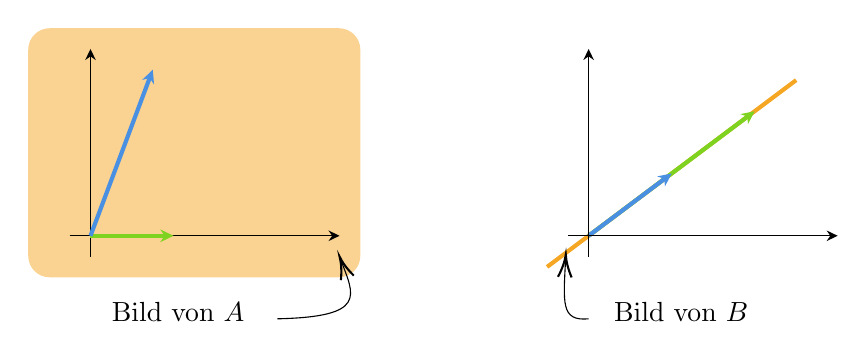
\begin{tikzpicture}[x=0.75pt,y=0.75pt,yscale=-1,xscale=1]
        %Straight Lines [id:da4469081308434383] 
        \draw [color={rgb, 255:red, 245; green, 166; blue, 35 }  ,draw opacity=1 ][line width=1.5]    (510,115) -- (390,205) ;
        %Rounded Rect [id:dp03142267072905092] 
        \draw  [draw opacity=0][fill={rgb, 255:red, 245; green, 166; blue, 35 }  ,fill opacity=0.5 ] (140,100.32) .. controls (140,94.62) and (144.62,90) .. (150.32,90) -- (289.68,90) .. controls (295.38,90) and (300,94.62) .. (300,100.32) -- (300,199.68) .. controls (300,205.38) and (295.38,210) .. (289.68,210) -- (150.32,210) .. controls (144.62,210) and (140,205.38) .. (140,199.68) -- cycle ;
        %Straight Lines [id:da10504323218580791] 
        \draw [color={rgb, 255:red, 126; green, 211; blue, 33 }  ,draw opacity=1 ][line width=1.5]    (410,190) -- (486.8,132.4) ;
        \draw [shift={(490,130)}, rotate = 143.13] [fill={rgb, 255:red, 126; green, 211; blue, 33 }  ,fill opacity=1 ][line width=0.08]  [draw opacity=0] (6.43,-3.09) -- (0,0) -- (6.43,3.09) -- (4.27,0) -- cycle    ;
        %Straight Lines [id:da4872975814697238] 
        \draw [color={rgb, 255:red, 74; green, 144; blue, 226 }  ,draw opacity=1 ][line width=1.5]    (410,190) -- (446.8,162.4) ;
        \draw [shift={(450,160)}, rotate = 143.13] [fill={rgb, 255:red, 74; green, 144; blue, 226 }  ,fill opacity=1 ][line width=0.08]  [draw opacity=0] (6.43,-3.09) -- (0,0) -- (6.43,3.09) -- (4.27,0) -- cycle    ;
        %Straight Lines [id:da29042899893351315] 
        \draw [color={rgb, 255:red, 0; green, 0; blue, 0 }  ,draw opacity=1 ]   (170,200) -- (170,103) ;
        \draw [shift={(170,100)}, rotate = 90] [fill={rgb, 255:red, 0; green, 0; blue, 0 }  ,fill opacity=1 ][line width=0.08]  [draw opacity=0] (5.36,-2.57) -- (0,0) -- (5.36,2.57) -- (3.56,0) -- cycle    ;
        %Straight Lines [id:da7550763838374285] 
        \draw [color={rgb, 255:red, 0; green, 0; blue, 0 }  ,draw opacity=1 ]   (160,190) -- (287,190) ;
        \draw [shift={(290,190)}, rotate = 180] [fill={rgb, 255:red, 0; green, 0; blue, 0 }  ,fill opacity=1 ][line width=0.08]  [draw opacity=0] (5.36,-2.57) -- (0,0) -- (5.36,2.57) -- (3.56,0) -- cycle    ;
        %Straight Lines [id:da3805155026706256] 
        \draw [color={rgb, 255:red, 126; green, 211; blue, 33 }  ,draw opacity=1 ][line width=1.5]    (170,190) -- (206,190) ;
        \draw [shift={(210,190)}, rotate = 180] [fill={rgb, 255:red, 126; green, 211; blue, 33 }  ,fill opacity=1 ][line width=0.08]  [draw opacity=0] (6.43,-3.09) -- (0,0) -- (6.43,3.09) -- (4.27,0) -- cycle    ;
        %Straight Lines [id:da5573776231790816] 
        \draw [color={rgb, 255:red, 74; green, 144; blue, 226 }  ,draw opacity=1 ][line width=1.5]    (170,190) -- (198.6,113.75) ;
        \draw [shift={(200,110)}, rotate = 110.56] [fill={rgb, 255:red, 74; green, 144; blue, 226 }  ,fill opacity=1 ][line width=0.08]  [draw opacity=0] (6.43,-3.09) -- (0,0) -- (6.43,3.09) -- (4.27,0) -- cycle    ;
        %Straight Lines [id:da5738079936769741] 
        \draw [color={rgb, 255:red, 0; green, 0; blue, 0 }  ,draw opacity=1 ]   (410,200) -- (410,103) ;
        \draw [shift={(410,100)}, rotate = 90] [fill={rgb, 255:red, 0; green, 0; blue, 0 }  ,fill opacity=1 ][line width=0.08]  [draw opacity=0] (5.36,-2.57) -- (0,0) -- (5.36,2.57) -- (3.56,0) -- cycle    ;
        %Straight Lines [id:da5379398767264265] 
        \draw [color={rgb, 255:red, 0; green, 0; blue, 0 }  ,draw opacity=1 ]   (400,190) -- (527,190) ;
        \draw [shift={(530,190)}, rotate = 180] [fill={rgb, 255:red, 0; green, 0; blue, 0 }  ,fill opacity=1 ][line width=0.08]  [draw opacity=0] (5.36,-2.57) -- (0,0) -- (5.36,2.57) -- (3.56,0) -- cycle    ;
        %Curve Lines [id:da6284955918264795] 
        \draw    (260,230) .. controls (303.65,229.03) and (297.12,218.96) .. (290.6,201.63) ;
        \draw [shift={(290,200)}, rotate = 70.02] [color={rgb, 255:red, 0; green, 0; blue, 0 }  ][line width=0.75]    (10.93,-3.29) .. controls (6.95,-1.4) and (3.31,-0.3) .. (0,0) .. controls (3.31,0.3) and (6.95,1.4) .. (10.93,3.29)   ;
        %Curve Lines [id:da29555342702504683] 
        \draw    (410,230) .. controls (396.35,231.3) and (397.91,222.14) .. (398.92,200.68) ;
        \draw [shift={(399,199)}, rotate = 92.53] [color={rgb, 255:red, 0; green, 0; blue, 0 }  ][line width=0.75]    (10.93,-3.29) .. controls (6.95,-1.4) and (3.31,-0.3) .. (0,0) .. controls (3.31,0.3) and (6.95,1.4) .. (10.93,3.29)   ;

        % Text Node
        \draw (179,221) node [anchor=north west][inner sep=0.75pt]   [align=left] {Bild von $\displaystyle A$ \ };
        % Text Node
        \draw (421,221) node [anchor=north west][inner sep=0.75pt]   [align=left] {Bild von $\displaystyle B$ \ };
    \end{tikzpicture}
\end{figure}   

Das Bild von \( A \) spannt den gesamten zweidimensionalen Raum auf, da die Spaltenvektoren linear unabhängig sind (zeigen in unterschiedliche Richtungen). Das Bild von \( B \), im Gegensatz, ist nur eine Linie da die Spaltenvektoren linear abhängig sind (zeigen in dieselbe Richtung). Dies stimmt auch mit der obigen Definition überein, denn

\begin{equation*}
    Ax =
    \begin{pmatrix}
        1 & 2 \\
        2 & 0 \\
    \end{pmatrix}
    \begin{pmatrix}
        x_1 \\
        x_2 \\
    \end{pmatrix} = \underbrace{ x_1
    \begin{pmatrix}
        1 \\
        2 \\
    \end{pmatrix} + x_2
    \begin{pmatrix}
        2 \\
        0 \\
    \end{pmatrix}}_{\text{linear unabhängig}},
\end{equation*}

\vspace{0.25\baselineskip}

\begin{equation*}
    Bx =
    \begin{pmatrix}
        1 & 2 \\
        2 & 4 \\
    \end{pmatrix}
    \begin{pmatrix}
        x_1 \\
        x_2 \\
    \end{pmatrix} = \underbrace{ x_1
    \begin{pmatrix}
        1 \\
        2 \\
    \end{pmatrix} + x_2
    \begin{pmatrix}
        2 \\
        4 \\
    \end{pmatrix}}_{\text{linear abhängig}}.
\end{equation*}

\vspace{0.25\baselineskip}

Wir können hier erkennen, dass die Dimension des Bildes gleich der Anzahl linear unabhängiger Spalten bzw.\ dem Rang der Matrix ist. Allgemein gilt:

\begin{equation*}
    \text{dim}(\text{Bild}(A)) = \text{Rang}(A).
\end{equation*}

\vspace{0.25\baselineskip}

\subsubsection*{Beispiel}

Oft muss ein Erzeugendensystem oder Basis des Bildes einer Matrix gefunden werden. Sei beispielsweise eine Matrix \( A \) gegeben durch:

\begin{equation*}
    A = \begin{pmatrix}
        1 & 2 & 4 \\
        3 & 1 & 5 \\
        4 & 3 & 9 \\
    \end{pmatrix}.
\end{equation*}

\begin{itemize}
    \item \textbf{Aufgabe:} Finden Sie ein Erzeugendensystem für das Bild von \( A \).
    
    Hier können wir einfach die Spaltenvektoren ablesen und erhalten
    \begin{equation*}
        \text{Bild}(A)=\left\{ \begin{pmatrix} 1 \\ 3 \\ 4 \\ \end{pmatrix}, \begin{pmatrix} 2 \\ 1 \\ 3 \\ \end{pmatrix}, \begin{pmatrix} 4 \\ 5 \\ 9 \\ \end{pmatrix} \right\}.
    \end{equation*}

    \item \textbf{Aufgabe:} Finden Sie eine Basis für das Bild von \( A \).
    
    Wir suchen nun alle linear unabhängigen Spalten von \( A \). Dafür transponieren wir die originale Matrix \( A \), wodurch die Spalten zu den Zeilen werden und umgekehrt. Nun wenden wir den Gauss-Algorithmus an und nehmen die Zeilen, die nicht Null sind, als Basis des Bildes. Wir erhalten:

    \begin{equation*}
        A^\top =
        \begin{pmatrix}
            1 & 3 & 4 \\
            2 & 1 & 3 \\
            4 & 5 & 9 \\
        \end{pmatrix} \xrightarrow{\text{Gauss}} \begin{pmatrix}
            1 & 3 & 4 \\
            0 & -5 & -5 \\
            0 & 0 & 0 \\
        \end{pmatrix}.
    \end{equation*}

    \vspace{0.25\baselineskip}

    Somit ist eine mögliche Basis gegeben durch 

    \begin{equation*}
        \text{Bild}(A)=\left\{ \begin{pmatrix} 1 \\ 3 \\ 4 \\ \end{pmatrix}, \begin{pmatrix} 0 \\ -5 \\ -5 \\ \end{pmatrix} \right\}.
    \end{equation*}

    \vspace{0.25\baselineskip}

    (Falls man direkt erkennt wie viele linear unabhängige Spalten eine Matrix hat, kann man ohne Rechnung die entsprechende Anzahl an linear unabhängigen Spaltenvektoren nehmen. Bei grossen Matrizen kann es aber schwierig sein, lineare Abhängigkeit zwischen Spalten zu erkennen.)

\end{itemize}

\subsection{Kern}

Um eine Intuition für den Kern zu bekommen, blicken wir nochmals auf das Bild einer Matrix. Das Bild beschreibt den Raum auf welchen alle beliebigen Vektoren \( x \) durch \( A \) abgebildet werden. Für die Matrix 

\begin{equation*}
    A = \begin{pmatrix}
        2 & 4 \\
        1 & 2 \\
    \end{pmatrix},
\end{equation*}

können wir uns das Bild grafisch als eine Linie vorstellen da \( A \) zwei linear abhängige Spalten hat. Betrachten wir nun was passiert, wenn einige Vektoren \( \textcolor{customlila}{v} \) durch \( A \) abgebildet werden, d.h.\ \( A \textcolor{customlila}{v} = \textcolor{customred}{u} \)

\begin{equation*}
    \begin{pmatrix}
        2 & 4 \\
        1 & 2 \\
    \end{pmatrix}
    \begin{pmatrix}
        2 \\
        0 \\
    \end{pmatrix} = 
    \begin{pmatrix}
        4 \\
        2 \\
    \end{pmatrix}\quad  \quad
    \begin{pmatrix}
        2 & 4 \\
        1 & 2 \\
    \end{pmatrix}
    \begin{pmatrix}
        0 \\
        \frac{1}{2} \\
    \end{pmatrix} = 
    \begin{pmatrix}
        2 \\
        1 \\
    \end{pmatrix}\quad  \quad
    \begin{pmatrix}
        2 & 4 \\
        1 & 2 \\
    \end{pmatrix}
    \begin{pmatrix}
        1 \\
        -1 \\
    \end{pmatrix} = 
    \begin{pmatrix}
        2 \\
        1 \\
    \end{pmatrix}.
\end{equation*}


\begin{figure*}[h]
    \centering
    \tikzset{every picture/.style={line width=0.75pt}} %set default line width to 0.75pt        
    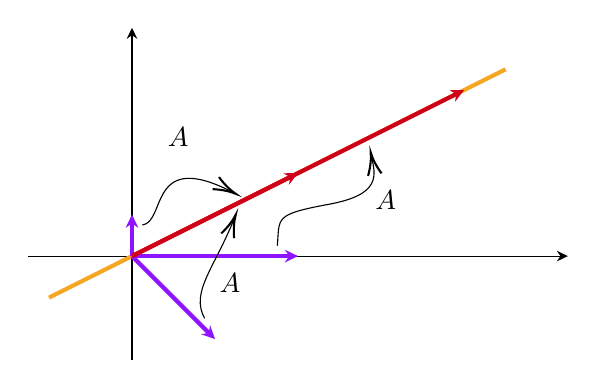
\begin{tikzpicture}[x=0.75pt,y=0.75pt,yscale=-1,xscale=1]
        %uncomment if require: \path (0,300); %set diagram left start at 0, and has height of 300
        %Straight Lines [id:da6593588772624016] 
        \draw [color={rgb, 255:red, 0; green, 0; blue, 0 }  ,draw opacity=1 ]   (220,180) -- (220,23) ;
        \draw [shift={(220,20)}, rotate = 90] [fill={rgb, 255:red, 0; green, 0; blue, 0 }  ,fill opacity=1 ][line width=0.08]  [draw opacity=0] (5.36,-2.57) -- (0,0) -- (5.36,2.57) -- (3.56,0) -- cycle    ;
        %Straight Lines [id:da3148050286568629] 
        \draw [color={rgb, 255:red, 0; green, 0; blue, 0 }  ,draw opacity=1 ]   (170,130) -- (427,130) ;
        \draw [shift={(430,130)}, rotate = 180] [fill={rgb, 255:red, 0; green, 0; blue, 0 }  ,fill opacity=1 ][line width=0.08]  [draw opacity=0] (5.36,-2.57) -- (0,0) -- (5.36,2.57) -- (3.56,0) -- cycle    ;
        %Straight Lines [id:da6808700521611847] 
        \draw [color={rgb, 255:red, 245; green, 166; blue, 35 }  ,draw opacity=1 ][line width=1.5]    (400,40) -- (180,150) ;
        %Straight Lines [id:da5600776280932787] 
        \draw [color={rgb, 255:red, 144; green, 19; blue, 254 }  ,draw opacity=1 ][line width=1.5]    (220,130) -- (296,130) ;
        \draw [shift={(300,130)}, rotate = 180] [fill={rgb, 255:red, 144; green, 19; blue, 254 }  ,fill opacity=1 ][line width=0.08]  [draw opacity=0] (6.43,-3.09) -- (0,0) -- (6.43,3.09) -- (4.27,0) -- cycle    ;
        %Straight Lines [id:da29159806020546475] 
        \draw [color={rgb, 255:red, 144; green, 19; blue, 254 }  ,draw opacity=1 ][line width=1.5]    (220,130) -- (220,114) ;
        \draw [shift={(220,110)}, rotate = 90] [fill={rgb, 255:red, 144; green, 19; blue, 254 }  ,fill opacity=1 ][line width=0.08]  [draw opacity=0] (6.43,-3.09) -- (0,0) -- (6.43,3.09) -- (4.27,0) -- cycle    ;
        %Straight Lines [id:da02904385361665396] 
        \draw [color={rgb, 255:red, 144; green, 19; blue, 254 }  ,draw opacity=1 ][line width=1.5]    (220,130) -- (257.17,167.17) ;
        \draw [shift={(260,170)}, rotate = 225] [fill={rgb, 255:red, 144; green, 19; blue, 254 }  ,fill opacity=1 ][line width=0.08]  [draw opacity=0] (6.43,-3.09) -- (0,0) -- (6.43,3.09) -- (4.27,0) -- cycle    ;
        %Straight Lines [id:da8418554959062283] 
        \draw [color={rgb, 255:red, 208; green, 2; blue, 27 }  ,draw opacity=1 ][line width=1.5]    (220,130) -- (376.42,51.79) ;
        \draw [shift={(380,50)}, rotate = 153.43] [fill={rgb, 255:red, 208; green, 2; blue, 27 }  ,fill opacity=1 ][line width=0.08]  [draw opacity=0] (6.43,-3.09) -- (0,0) -- (6.43,3.09) -- (4.27,0) -- cycle    ;
        %Straight Lines [id:da2776418785515896] 
        \draw [color={rgb, 255:red, 208; green, 2; blue, 27 }  ,draw opacity=1 ][line width=1.5]    (220,130) -- (296.42,91.79) ;
        \draw [shift={(300,90)}, rotate = 153.43] [fill={rgb, 255:red, 208; green, 2; blue, 27 }  ,fill opacity=1 ][line width=0.08]  [draw opacity=0] (6.43,-3.09) -- (0,0) -- (6.43,3.09) -- (4.27,0) -- cycle    ;
        %Curve Lines [id:da5723820162810079] 
        \draw    (290,125) .. controls (291.25,111.5) and (288,110) .. (315,105) .. controls (340.25,100.33) and (337.33,91) .. (335.38,81.89) ;
        \draw [shift={(335,80)}, rotate = 79.55] [color={rgb, 255:red, 0; green, 0; blue, 0 }  ][line width=0.75]    (10.93,-3.29) .. controls (6.95,-1.4) and (3.31,-0.3) .. (0,0) .. controls (3.31,0.3) and (6.95,1.4) .. (10.93,3.29)   ;
        %Curve Lines [id:da27604530152523477] 
        \draw    (225,115) .. controls (236.63,113.52) and (227.68,77.97) .. (268.74,99.34) ;
        \draw [shift={(270,100)}, rotate = 208.16] [color={rgb, 255:red, 0; green, 0; blue, 0 }  ][line width=0.75]    (10.93,-3.29) .. controls (6.95,-1.4) and (3.31,-0.3) .. (0,0) .. controls (3.31,0.3) and (6.95,1.4) .. (10.93,3.29)   ;
        %Curve Lines [id:da2649828745139027] 
        \draw    (255,160) .. controls (247.93,147.32) and (259.88,135.6) .. (269.28,111.85) ;
        \draw [shift={(270,110)}, rotate = 110.81] [color={rgb, 255:red, 0; green, 0; blue, 0 }  ][line width=0.75]    (10.93,-3.29) .. controls (6.95,-1.4) and (3.31,-0.3) .. (0,0) .. controls (3.31,0.3) and (6.95,1.4) .. (10.93,3.29)   ;

        % Text Node
        \draw (336,97) node [anchor=north west][inner sep=0.75pt]   [align=left] {$\displaystyle A$};
        % Text Node
        \draw (236,67) node [anchor=north west][inner sep=0.75pt]   [align=left] {$\displaystyle A$};
        % Text Node
        \draw (261,137) node [anchor=north west][inner sep=0.75pt]   [align=left] {$\displaystyle A$};
    \end{tikzpicture}
\end{figure*}

Man erkennt, dass alle Vektoren nach der Multiplikation mit \( A \) wie erwartet im \textcolor{customorange}{Bild} liegen (in diesem fall auf der orangen Linie). Wir können uns nun fragen welche Vektoren \( \textcolor{customblue}{x} \) durch \( A \) auf null abgebildet werden. D.h.\ wir suchen all \( \textcolor{customblue}{x} \), sodass \( A \textcolor{customblue}{x} = \textcolor{customred}{0} \). Zum Beispiel erfüllen diese Vektoren die Bedingung:

\begin{equation*}
    \begin{pmatrix}
        2 & 4 \\
        1 & 2 \\
    \end{pmatrix}
    \begin{pmatrix}
        2 \\
        -1 \\
    \end{pmatrix} = 
    \begin{pmatrix}
        0 \\
        0 \\
    \end{pmatrix}\quad  \quad
    \begin{pmatrix}
        2 & 4 \\
        1 & 2 \\
    \end{pmatrix}
    \begin{pmatrix}
        -2 \\
        1 \\
    \end{pmatrix} = 
    \begin{pmatrix}
        0 \\
        0 \\
    \end{pmatrix}\quad  \quad
    \begin{pmatrix}
        2 & 4 \\
        1 & 2 \\
    \end{pmatrix}
    \begin{pmatrix}
        4 \\
        -2 \\
    \end{pmatrix} = 
    \begin{pmatrix}
        0 \\
        0 \\
    \end{pmatrix}.
\end{equation*}

\begin{figure*}[h]
    \centering
    \tikzset{every picture/.style={line width=0.75pt}} %set default line width to 0.75pt        
    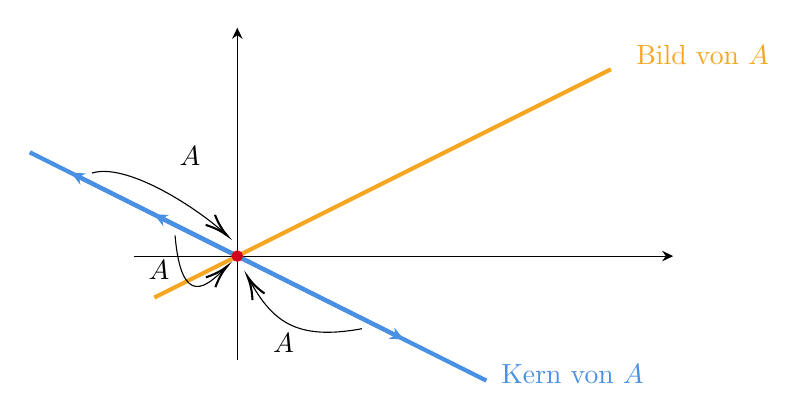
\begin{tikzpicture}[x=0.75pt,y=0.75pt,yscale=-1,xscale=1]
        %uncomment if require: \path (0,300); %set diagram left start at 0, and has height of 300
        %Straight Lines [id:da6593588772624016] 
        \draw [color={rgb, 255:red, 0; green, 0; blue, 0 }  ,draw opacity=1 ]   (220,180) -- (220,23) ;
        \draw [shift={(220,20)}, rotate = 90] [fill={rgb, 255:red, 0; green, 0; blue, 0 }  ,fill opacity=1 ][line width=0.08]  [draw opacity=0] (5.36,-2.57) -- (0,0) -- (5.36,2.57) -- (3.56,0) -- cycle    ;
        %Straight Lines [id:da3148050286568629] 
        \draw [color={rgb, 255:red, 0; green, 0; blue, 0 }  ,draw opacity=1 ]   (170,130) -- (427,130) ;
        \draw [shift={(430,130)}, rotate = 180] [fill={rgb, 255:red, 0; green, 0; blue, 0 }  ,fill opacity=1 ][line width=0.08]  [draw opacity=0] (5.36,-2.57) -- (0,0) -- (5.36,2.57) -- (3.56,0) -- cycle    ;
        %Straight Lines [id:da6808700521611847] 
        \draw [color={rgb, 255:red, 245; green, 166; blue, 35 }  ,draw opacity=1 ][line width=1.5]    (400,40) -- (180,150) ;
        %Curve Lines [id:da27604530152523477] 
        \draw    (150,90) .. controls (166.01,84.91) and (198.48,105.22) .. (213.64,118.76) ;
        \draw [shift={(215,120)}, rotate = 222.95] [color={rgb, 255:red, 0; green, 0; blue, 0 }  ][line width=0.75]    (10.93,-3.29) .. controls (6.95,-1.4) and (3.31,-0.3) .. (0,0) .. controls (3.31,0.3) and (6.95,1.4) .. (10.93,3.29)   ;
        %Curve Lines [id:da2649828745139027] 
        \draw    (280,165) .. controls (248.07,170.85) and (236.81,161.25) .. (225.84,141.54) ;
        \draw [shift={(225,140)}, rotate = 61.53] [color={rgb, 255:red, 0; green, 0; blue, 0 }  ][line width=0.75]    (10.93,-3.29) .. controls (6.95,-1.4) and (3.31,-0.3) .. (0,0) .. controls (3.31,0.3) and (6.95,1.4) .. (10.93,3.29)   ;
        %Straight Lines [id:da0086549162933367] 
        \draw [color={rgb, 255:red, 74; green, 144; blue, 226 }  ,draw opacity=1 ][line width=1.5]    (340,190) -- (120,80) ;
        %Straight Lines [id:da5600776280932787] 
        \draw [color={rgb, 255:red, 74; green, 144; blue, 226 }  ,draw opacity=1 ][line width=1.5]    (220,130) -- (183.58,111.79) ;
        \draw [shift={(180,110)}, rotate = 26.57] [fill={rgb, 255:red, 74; green, 144; blue, 226 }  ,fill opacity=1 ][line width=0.08]  [draw opacity=0] (6.43,-3.09) -- (0,0) -- (6.43,3.09) -- (4.27,0) -- cycle    ;
        %Straight Lines [id:da29159806020546475] 
        \draw [color={rgb, 255:red, 74; green, 144; blue, 226 }  ,draw opacity=1 ][line width=1.5]    (220,130) -- (143.58,91.79) ;
        \draw [shift={(140,90)}, rotate = 26.57] [fill={rgb, 255:red, 74; green, 144; blue, 226 }  ,fill opacity=1 ][line width=0.08]  [draw opacity=0] (6.43,-3.09) -- (0,0) -- (6.43,3.09) -- (4.27,0) -- cycle    ;
        %Straight Lines [id:da02904385361665396] 
        \draw [color={rgb, 255:red, 74; green, 144; blue, 226 }  ,draw opacity=1 ][line width=1.5]    (220,130) -- (296.42,168.21) ;
        \draw [shift={(300,170)}, rotate = 206.57] [fill={rgb, 255:red, 74; green, 144; blue, 226 }  ,fill opacity=1 ][line width=0.08]  [draw opacity=0] (6.43,-3.09) -- (0,0) -- (6.43,3.09) -- (4.27,0) -- cycle    ;
        %Curve Lines [id:da12414115273691662] 
        \draw    (190,120) .. controls (193.07,156.15) and (205.74,144.07) .. (213.67,136.3) ;
        \draw [shift={(215,135)}, rotate = 135.94] [color={rgb, 255:red, 0; green, 0; blue, 0 }  ][line width=0.75]    (10.93,-3.29) .. controls (6.95,-1.4) and (3.31,-0.3) .. (0,0) .. controls (3.31,0.3) and (6.95,1.4) .. (10.93,3.29)   ;
        %Shape: Circle [id:dp6898749088101324] 
        \draw  [color={rgb, 255:red, 208; green, 2; blue, 27 }  ,draw opacity=1 ][fill={rgb, 255:red, 208; green, 2; blue, 27 }  ,fill opacity=1 ] (217.5,130) .. controls (217.5,128.62) and (218.62,127.5) .. (220,127.5) .. controls (221.38,127.5) and (222.5,128.62) .. (222.5,130) .. controls (222.5,131.38) and (221.38,132.5) .. (220,132.5) .. controls (218.62,132.5) and (217.5,131.38) .. (217.5,130) -- cycle ;

        % Text Node
        \draw (176,131) node [anchor=north west][inner sep=0.75pt]   [align=left] {$\displaystyle A$};
        % Text Node
        \draw (191,76) node [anchor=north west][inner sep=0.75pt]   [align=left] {$\displaystyle A$};
        % Text Node
        \draw (236,166) node [anchor=north west][inner sep=0.75pt]   [align=left] {$\displaystyle A$};
        % Text Node
        \draw (411,27) node [anchor=north west][inner sep=0.75pt]  [color={rgb, 255:red, 245; green, 166; blue, 35 }  ,opacity=1 ] [align=left] {Bild von $\displaystyle A$};
        % Text Node
        \draw (346,181) node [anchor=north west][inner sep=0.75pt]  [color={rgb, 255:red, 74; green, 144; blue, 226 }  ,opacity=1 ] [align=left] {Kern von $\displaystyle A$};
    \end{tikzpicture}
\end{figure*}

\vspace{0.5\baselineskip}

Wir erkennen, dass alle Vektoren auf der blauen Linie diese Bedingung erfüllen. Diese resultierende Menge, aller Vektoren, die auf null abgebildet werden, wird Kern genannt. Diese Menge ist äquivalent zur Lösung des HLGS \( Ax = 0 \). Mathematisch ausgedrückt ist der Kern einer Matrix \( A \) definiert durch

\begin{equation*}
    \text{Kern}(A) = \{ x \in \mathbb{R}^n \mid Ax = 0 \}.
\end{equation*}

Mit der Definition von Kern können wir auch die im ersten Abschnitt eingeführte Zusammenhangs-Liste ergänzen. 

\begin{tcolorbox}[colback=gray!30, colframe=gray!80, title=Wichtige Zusammenhänge]
    Folgende Aussagen sind für \( A \in \mathbb{R}^{n \times n} \) äquivalent:
    \begin{itemize}
        \item \(rang (A) = n \)
        \item Das LGS \( Ax=b \) ist für beliebiges \( b \) lösbar
        \item Das LGS \( Ax=b \) hat genau eine Lösung
        \item Das homogene LGS \( Ax=0 \) hat nur die triviale Lösung \( x = 0 \)
        \item Die Zeilen und Spalten von \( A \) sind linear unabhängig
        \item \( A \) ist invertierbar (regulär, nicht singulär)
        \item \( det(A) \neq 0 \)
        \item Die Spalten von \( A \) bilden eine Basis von \( \mathbb{R}^n \)
        \item \textcolor{red}{Der Kern besteht nur aus dem Nullvektor}
        \item \textcolor{red}{Kein Eigenwert von \( A \) ist Null}
    \end{itemize}
\end{tcolorbox}

\vspace{0.5\baselineskip}

Um den Zusammenhang mit Eigenwerten zu verstehen, erinnern wir uns nochmals was Eigenwerte und Eigenvektoren sind. Ein Eigenvektor ist ein Vektor, der durch eine Multiplikation mit einer Matrix nur um einen Faktor \( \lambda \), dem Eigenwert, skaliert wird. Wenn nun ein Eigenwert Null ist, dann gibt es Vektoren (die nicht der Nullvektor sind) welche auf null abgebildet werden. D.h.\ das HLGS \( Ax = 0 \) hat nicht triviale Lösungen \( x \neq 0 \) und dadurch ist der Rang der Matrix nicht voll.

\subsubsection*{Beispiel}

\begin{itemize}
    \item Bestimme den Kern der Matrix
    \begin{equation*}
        A = \begin{pmatrix} 2 & 4 \\ 1 & 2 \end{pmatrix}
    \end{equation*}
    Löse das HLGS \( Ax = 0 \):
    \begin{equation*}
        \begin{array}{cc|c}
            2 & 4 & 0 \\
            1 & 2 & 0 \\
        \end{array} \xrightarrow{\text{Gauss}}
        \begin{array}{cc|c}
            2 & 4 & 0 \\
            0 & 0 & 0 \\
        \end{array} \qquad
        \begin{aligned}
            x_2 &= t \\
            x_1 &= -2t 
        \end{aligned} \quad \rightarrow \quad \text{Kern}(A) = \text{span} \left\{ 
        \begin{pmatrix}
            -2 \\ 1 
        \end{pmatrix} \right\}
    \end{equation*} 
\end{itemize}

\subsection{Beziehung zwischen Kern und Bild}

Im Folgenden wollen wir Zusammenhänge zwischen Kern und Bild genauer betrachten. Spezifischer wollen wir zwei wichtige Eigenschaften beweisen. Die erste Eigenschaft 

\begin{equation*}
    i. \quad \text{dim}(\text{Kern}) + \text{dim}(\text{Bild}) = n,
        % ii. & \quad \text{Kern}(A^\top) \perp \text{Bild}(A).
\end{equation*}

lässt sich sowohl grafisch als auch mathematisch Beweisen. 

\subsubsection*{Grafische Intuition} \( \quad \)

Beginnen wir mit dem grafischen Beweis in 2 Dimensionen. Sei \( A \in \mathbb{R}^{m \times n} \) und \( \textcolor{customlila}{v} \in \mathbb{R}^n \) ein beliebiger Vektor. Ausserdem sei \( A \textcolor{customlila}{v} = \textcolor{customgreen}{w} \). Wir können nun \( \textcolor{customlila}{v} \) in zwei Komponenten zerlegen:

\begin{equation*}
    \textcolor{customlila}{v} = \textcolor{customred}{\hat{v}} + \textcolor{customred}{\bar{v}} \quad \left\{
    \begin{aligned}
        & \textcolor{customred}{\hat{v}} \in \textcolor{customblue}{\text{Kern}(A)} \\[0.5em]
        & \textcolor{customred}{\bar{v}} \ \text{orthogonal zu} \ \textcolor{customred}{\hat{v}}
    \end{aligned}
    \right.
\end{equation*}

Dadurch ist:

\begin{equation*}
    A \textcolor{customlila}{v} = A ( \textcolor{customred}{\hat{v}} + \textcolor{customred}{\bar{v}} ) = \cancelto{0}{A \textcolor{customred}{\hat{v}}} + A \textcolor{customred}{\bar{v}} = A \textcolor{customred}{\bar{v}} = \textcolor{customgreen}{w}.
\end{equation*}

Der Term \( A \textcolor{customred}{\hat{v}} \) ist Null, da \( \textcolor{customred}{\hat{v}} \) im Kern von \( A \) liegt. Letztlich definieren wir noch einen zum Kern orthogonalen Unterraum \( \textcolor{custombrown}{U} \). Per Definition ist dadurch \( \textcolor{customred}{\bar{v}} \in \textcolor{custombrown}{U} \). Zusammengefasst können wir das ganze grafisch darstellen:

\begin{figure*}[h]
    \centering
    \tikzset{every picture/.style={line width=0.75pt}} %set default line width to 0.75pt        

    \begin{tikzpicture}[x=0.75pt,y=0.75pt,yscale=-1,xscale=1]
        %uncomment if require: \path (0,300); %set diagram left start at 0, and has height of 300
        %Straight Lines [id:da5180488228733903] 
        \draw [color={rgb, 255:red, 0; green, 0; blue, 0 }  ,draw opacity=1 ]   (249.02,276.33) -- (249.02,22.83) ;
        \draw [shift={(249.02,19.83)}, rotate = 90] [fill={rgb, 255:red, 0; green, 0; blue, 0 }  ,fill opacity=1 ][line width=0.08]  [draw opacity=0] (5.36,-2.57) -- (0,0) -- (5.36,2.57) -- (3.56,0) -- cycle    ;
        %Straight Lines [id:da6154875232624479] 
        \draw [color={rgb, 255:red, 0; green, 0; blue, 0 }  ,draw opacity=1 ]   (140.67,168.33) -- (498.84,168.33) ;
        \draw [shift={(501.84,168.33)}, rotate = 180] [fill={rgb, 255:red, 0; green, 0; blue, 0 }  ,fill opacity=1 ][line width=0.08]  [draw opacity=0] (5.36,-2.57) -- (0,0) -- (5.36,2.57) -- (3.56,0) -- cycle    ;
        %Straight Lines [id:da7707590578093849] 
        \draw [color={rgb, 255:red, 245; green, 166; blue, 35 }  ,draw opacity=1 ][line width=1.5]    (309.22,33.33) -- (212.9,249.33) ;
        %Straight Lines [id:da5279464933698] 
        \draw [color={rgb, 255:red, 74; green, 144; blue, 226 }  ,draw opacity=1 ][line width=1.5]    (489.8,100.83) -- (152.71,195.33) ;
        %Straight Lines [id:da46864676376854864] 
        \draw [color={rgb, 255:red, 139; green, 87; blue, 42 }  ,draw opacity=1 ][line width=1.5]    (218.92,33.33) -- (267.08,249.33) ;
        %Straight Lines [id:da7574921043857895] 
        \draw [color={rgb, 255:red, 208; green, 2; blue, 27 }  ,draw opacity=1 ][line width=1.5]    (249.02,168.33) -- (341.48,142.4) ;
        \draw [shift={(345.33,141.32)}, rotate = 164.34] [fill={rgb, 255:red, 208; green, 2; blue, 27 }  ,fill opacity=1 ][line width=0.08]  [draw opacity=0] (6.43,-3.09) -- (0,0) -- (6.43,3.09) -- (4.27,0) -- cycle    ;
        %Straight Lines [id:da2817526342161202] 
        \draw [color={rgb, 255:red, 208; green, 2; blue, 27 }  ,draw opacity=1 ][line width=1.5]    (249.02,168.33) -- (237.85,118.23) ;
        \draw [shift={(236.98,114.33)}, rotate = 77.43] [fill={rgb, 255:red, 208; green, 2; blue, 27 }  ,fill opacity=1 ][line width=0.08]  [draw opacity=0] (6.43,-3.09) -- (0,0) -- (6.43,3.09) -- (4.27,0) -- cycle    ;
        %Straight Lines [id:da6422691947003276] 
        \draw [color={rgb, 255:red, 144; green, 19; blue, 254 }  ,draw opacity=1 ][line width=1.5]    (249.02,168.33) -- (330.41,90.1) ;
        \draw [shift={(333.29,87.33)}, rotate = 136.14] [fill={rgb, 255:red, 144; green, 19; blue, 254 }  ,fill opacity=1 ][line width=0.08]  [draw opacity=0] (6.43,-3.09) -- (0,0) -- (6.43,3.09) -- (4.27,0) -- cycle    ;
        %Straight Lines [id:da22124858854815466] 
        \draw [color={rgb, 255:red, 126; green, 211; blue, 33 }  ,draw opacity=1 ][line width=1.5]    (249.02,168.33) -- (295.55,63.98) ;
        \draw [shift={(297.18,60.33)}, rotate = 114.03] [fill={rgb, 255:red, 126; green, 211; blue, 33 }  ,fill opacity=1 ][line width=0.08]  [draw opacity=0] (6.43,-3.09) -- (0,0) -- (6.43,3.09) -- (4.27,0) -- cycle    ;
        %Straight Lines [id:da08466314042691692] 
        \draw [color={rgb, 255:red, 144; green, 19; blue, 254 }  ,draw opacity=1 ][line width=0.75]  [dash pattern={on 0.84pt off 2.51pt}]  (236.98,114.33) -- (333.29,87.33) ;
        %Straight Lines [id:da5962898587865522] 
        \draw [color={rgb, 255:red, 144; green, 19; blue, 254 }  ,draw opacity=1 ][line width=0.75]  [dash pattern={on 0.84pt off 2.51pt}]  (345.33,141.32) -- (333.29,87.33) ;

        % Text Node
        \draw (317.66,12) node [anchor=north west][inner sep=0.75pt]  [color={rgb, 255:red, 245; green, 166; blue, 35 }  ,opacity=1 ] [align=left] {Bild von $\displaystyle A$};
        % Text Node
        \draw (435,75) node [anchor=north west][inner sep=0.75pt]  [color={rgb, 255:red, 74; green, 144; blue, 226 }  ,opacity=1 ] [align=left] {Kern von $\displaystyle A$};
        % Text Node
        \draw (275,242) node [anchor=north west][inner sep=0.75pt]  [color={rgb, 255:red, 139; green, 87; blue, 42 }  ,opacity=1 ] [align=left] {$\displaystyle U$};
        % Text Node
        \draw (343,148) node [anchor=north west][inner sep=0.75pt]  [color={rgb, 255:red, 208; green, 2; blue, 27 }  ,opacity=1 ] [align=left] {\( \textcolor{customred}{\hat{v}} \)};
        % Text Node
        \draw (218,113) node [anchor=north west][inner sep=0.75pt]  [color={rgb, 255:red, 208; green, 2; blue, 27 }  ,opacity=1 ] [align=left] {\( \textcolor{customred}{\bar{v}} \)};
        % Text Node
        \draw (337,74) node [anchor=north west][inner sep=0.75pt]  [color={rgb, 255:red, 144; green, 19; blue, 254 }  ,opacity=1 ] [align=left] {$\displaystyle v$};
          % Text Node
          \draw (270,60) node [anchor=north west][inner sep=0.75pt]  [color={rgb, 255:red, 208; green, 2; blue, 27 }  ,opacity=1 ] [align=left] {\( \textcolor{customgreen}{w} \)};
    \end{tikzpicture}
\end{figure*}

Folgende Beobachtungen können nun gemacht werden:

\begin{itemize}
    \item Der \textcolor{customblue}{\text{Kern}} und der zum Kern orthogonale Unterraum \( \textcolor{custombrown}{U} \) haben zusammen die Dimension \( n \), da wir durch die Summe \( \textcolor{customlila}{v} = \textcolor{customred}{\hat{v}} + \textcolor{customred}{\bar{v}} \) alle Vektoren \( \textcolor{customlila}{v} \) erzeugen können.
    
    \begin{equation*}
        \text{dim}(\textcolor{customblue}{\text{Kern}}) + \text{dim}(\textcolor{custombrown}{U}) = n.
    \end{equation*}

    \item Jeder Vektor \( \textcolor{customred}{\bar{v}} \) in \( \textcolor{custombrown}{U} \) korrespondiert zu einem Vektor in \( \textcolor{customorange}{\text{Bild}} \) und umgekehrt, da \( A \textcolor{customred}{\bar{v}} = \textcolor{customgreen}{w} \). Die Dimension von \( \textcolor{custombrown}{U} \) ist also gleich der Dimension des \( \textcolor{customorange}{\text{Bildes}} \).
    
    \begin{equation*}
        \text{dim}(\textcolor{custombrown}{U}) = \text{dim}(\textcolor{customorange}{\text{Bild}}).
    \end{equation*}
\end{itemize}

Zusammen gilt also 
\begin{equation*}
    \text{dim}(\text{Kern}) + \text{dim}(\text{Bild}) = n.    
\end{equation*}

\subsubsection*{Mathematisch} \( \quad \)

Sei \( A \in \mathbb{R}^{m \times n} \) und der Kern per Definition die Lösungsmenge des HLGS \( Ax = 0 \). Diese Lösungsmenge hat \( n-r \) freie Parameter. Dabei ist \( r \) der Rang von \( A \) (Anzahl Pivots). Betrachten folgendes Beispiel:

\begin{equation*}
    A = \begin{pmatrix} 1 & 2 &  4 \\ 3 & 1 & 5 \\ 4 & 3 & 9 \end{pmatrix} \quad \xrightarrow{\text{HLGS}} \quad \begin{array}{ccc|c}
        1 & 2 & 4 & 0 \\
        3 & 1 & 5 & 0 \\
        4 & 3 & 9 & 0 \\
    \end{array} \quad \xrightarrow{\text{Gauss}} \quad \begin{array}{ccc|c}
        1 & 2 & 4 & 0 \\
        0 & -5 & -7 & 0 \\
        0 & 0 & 0 & 0 \\
    \end{array}
\end{equation*}

wodurch:

\begin{equation*}
    x_3 = t, \quad x_2 = -\frac{7}{5} t, \quad x_1 =  - \frac{6}{5}t;
\end{equation*}

und 

\begin{equation*}
    r = 2, \quad n = 3, \quad n - r = 1.
\end{equation*}

Der Lösungsraum von \( Ax=0 \) hat also die Dimension 1. Damit hat auch der Kern die Dimension 1. 

\begin{equation*}
    \text{dim}(\text{Kern}) = n - r.
\end{equation*}

Durch das Gauss-Verfahren haben wir bereits die Zeilenstufenform \( R \) von \( A \) gefunden. Die Bilder von \( A \) und \( R \) lassen sich durch die jeweiligen Spalten beschreiben

\begin{equation*}
    A = \begin{pmatrix}
        1 & 2 & 4 \\ 3 & 1 & 5 \\ 4 & 3 & 9
    \end{pmatrix} \qquad \qquad \qquad \qquad \quad
    R = \begin{pmatrix}
        1 & 2 & 4 \\ 0 & -5 & -7 \\ 0 & 0 & 0
    \end{pmatrix}
\end{equation*}

\vspace{0.5\baselineskip}

\begin{equation*}
    \text{Bild}(A) = \text{span} \left\{ a^{(1)}, a^{(2)}, a^{(3)} \right\} \quad \textcolor{customred}{\overset{!}{=}} \quad
    \text{Bild}(R) = \text{span} \left\{ r^{(1)}, r^{(2)}, r^{(3)} \right\}
\end{equation*}

\vspace{0.5\baselineskip}

Da \( A \) und \( R \) dieselbe Lösungsmenge beschreiben, spannen sie auch dasselbe Bild auf und haben auch dieselbe Dimension. Die Dimension von \( \text{Bild}(R) \) ist einfach zu bestimmen da sie gleich dem Rang \( r \) ist. Es gilt also 

\begin{equation*}
    \text{dim}(\text{Bild}(A)) = \text{dim}(\text{Bild}(R)) = r.
\end{equation*}

Dadurch ist

\begin{equation*}
    \text{dim}(\text{Kern}) + \text{dim}(\text{Bild}) = n - r + r = n, 
\end{equation*}

und somit

\begin{equation*}
    \text{dim}(\text{Kern}) + \text{dim}(\text{Bild}) = n. 
\end{equation*}

\newpage

Die zweite Eigenschaft, die wir beweisen wollen ist, gegeben durch:

\begin{equation*}
    ii. \quad \text{Kern}(A^\top) \perp \text{Bild}(A).
\end{equation*}

Den Beweis dazu können wir durch folgende Überlegung erlangen. Sei \( A \) definiert durch:

\begin{equation*}
    A = \begin{pmatrix}
        \vdots & \vdots & \vdots \\
        a^{(1)} & a^{(2)} & a^{(3)} \\
        \vdots & \vdots & \vdots
    \end{pmatrix}
\end{equation*}

wobei \( a^{(n)} \) die Spalten von \( A \) sind. Dadurch gilt das \( \text{Bild}(A) = \left\{ a^{(1)}, a^{(2)}, a^{(3)} \right\} \). Durch das Transponieren werden die Spalten \( a^{(n)} \) zu den Zeilen \( a^{[n]} \). 

\begin{equation*}
    A^\top = \begin{pmatrix}
        \cdots & a^{[1]} & \cdots \\
        \cdots & a^{[2]} & \cdots \\
        \cdots & a^{[3]} & \cdots \\
    \end{pmatrix}
\end{equation*}

Betrachten wir nun das HLGS \( A^\top y = 0 \). Allgemein ist dies definiert durch

\begin{equation*}
    A^\top y = \begin{pmatrix}
        \cdots & a^{[1]} & \cdots \\
        \cdots & a^{[2]} & \cdots \\
        \cdots & a^{[3]} & \cdots \\
    \end{pmatrix} \begin{pmatrix}
        y_1 \\ y_2 \\ y_3
    \end{pmatrix} = \begin{pmatrix}
        0 \\ 0 \\ 0
    \end{pmatrix}.
\end{equation*}

Wir sehen, dass der Vektor \( y \) immer im Kern von \( A^\top \) liegen muss, um diese Gleichung zu erfüllen. Nun können wir das Produkt von \( A^\top \) mit \( y \) auch als das Skalarprodukt von den Spalten \( a^{(n)} \) mit dem Vektor \( y \) interpretieren. Dieses Skalarprodukt \( \langle a^{(n)}, y \rangle \) ist immer Null, woraus folgt:

\begin{equation*}
    \text{Kern}(A^\top) \perp \text{Bild}(A).
\end{equation*}

Aus dieser Bedingung folgt die Fredholm Alternative welche besagt, dass \( Ax = b \) lösbar ist (\(b \) liegt im Bild) genau dann, wenn \( b \) senkrecht auf allen Lösungen des adjungierten LGS \( A^\top y = 0 \) steht.
